%%%%%%%%%%%%%%%%%%%%%%%%%%%%%%%%%%%%%%%%%%%%%%%%%%%%%%%%%%%%%%%%%%%%%%%%%%%
%%  chapter3.tex  –  Chapter 3: Instantiation of the Hybrid IDPS System
%%                              for Network Traffic Protection and Its
%%                              Benchmark Validation (with preliminary
%%                              extension to the UAV sector)
%%  v12 (Phase 2.5) – Merge of former Chapter 3 (instantiation) and
%%                    former Chapter 4 \S\S4.1-4.5 (methodology + NIDS
%%                    benchmark validation) into a single chapter.
%%                    Cross-cutting experiments remain in
%%                    Chapter~\ref{ch:experiments}.
%%%%%%%%%%%%%%%%%%%%%%%%%%%%%%%%%%%%%%%%%%%%%%%%%%%%%%%%%%%%%%%%%%%%%%%%%%%

\chapter{Instantiation of the Hybrid~IDPS System for Network Traffic Protection and Its Benchmark Validation}
\label{ch:adaptation}

This chapter systematically instantiates and validates the
\emph{system} Hybrid~IDPS formalised in Chapter~\ref{ch:methods} for
the network-traffic-protection sector
(\S\ref{subsubsec:sector_nids}). The chapter consists of two
methodologically linked parts. The \emph{first part}
(\S\ref{sec:nidps_context}--\S\ref{sec:integrated_arch})
systematically instantiates the tuple~\eqref{eq:hybrid_idps_tuple}
with the concrete entities of network security: NIDS-specific
terminologies are defined, together with the pipeline for
transforming raw traffic into a temporal graph, a unified
classification taxonomy of 34 threat classes, the engineering
pipeline for the 83-dimensional flow feature vector, the
hyperparameter configuration, and the integrated system
architecture. The \emph{second part}
(\S\ref{sec:exp_methodology}--\S\ref{sec:ablation}) systematically
validates the resulting instantiated system on six benchmark
datasets totalling 84.2 million labelled samples: it presents the
experimental methodology, the unified benchmark results, the
per-Model results for each of the seven Models M1--M7, the
comparison with baselines, and the ablation studies. The chapter
concludes with Chapter~\ref{ch:uav}~--- a \emph{preliminary
extension} of the Hybrid~IDPS system to the UAV sector, which
demonstrates the system's domain-independence as a preamble to the
full experimental programme for UAVs in Chapter~\ref{ch:uav}. The
cross-cutting validation of the Hybrid~IDPS system (adversarial
robustness across six attack families, cross-domain transfer to
speech and healthcare, post-quantum compatibility) is presented
separately in Chapter~\ref{ch:experiments}.

%%=====================================================================
\section{Problem Statement of Constructing an Adversarially Robust Hybrid IDPS for Network Traffic Analysis}
\label{sec:nidps_context}
%%====

\subsection{Hybrid Intrusion Detection and Prevention Systems}

A hybrid intrusion detection and prevention system (HIDPS)~\cite{Buczak2016,Ahmad2021,Aldweesh2020,Ferrag2020,Paxson1999} combines two complementary detection paradigms. Signature-based detection matches incoming traffic against a database of known patterns (rules) and achieves high precision on previously catalogued threats but cannot detect novel attacks. Anomaly-based detection learns a statistical model of normal behaviour and flags deviations, enabling detection of zero-day exploits and evolving attack patterns at the cost of potentially higher false-positive rates. The dissertation's methods operate within the anomaly-based branch, augmented by large language model reasoning for zero-shot classification of novel categories.

A Network IDPS (NIDPS) monitors traffic at the network layer, analysing flows and packets between hosts rather than events within a single endpoint. The three operating conditions of the architectural framework (Figure~\ref{fig:dissertation_architecture}) are all present in this domain: adversarial manipulation by deliberate opponents who craft traffic to evade detection, non-stationarity through evolving traffic patterns and protocol changes, and distribution of the monitoring infrastructure across organisational boundaries.

\subsection{Key Terminologies}

The following terms are used throughout this chapter and the experimental validation in Chapter~\ref{ch:experiments}:

\noindent\textbf{Flow.} A sequence of packets sharing a common 5-tuple (source IP, destination IP, source port, destination port, protocol). A flow is the fundamental unit of analysis and corresponds to a directed edge in the network graph.

\noindent\textbf{Session.} A bidirectional communication comprising a forward flow and its reverse counterpart, capturing the full exchange between two endpoints.

\noindent\textbf{Host.} A network endpoint (IP address) that participates as either source or destination. Hosts correspond to nodes in the network graph.

\noindent\textbf{Service.} A functional component identified by port number and protocol (e.g., HTTP on port 80, SSH on port 22). In cloud-native deployments, services correspond to microservice containers.

\noindent\textbf{PCAP (Packet Capture).} The raw binary format capturing full packet headers and optionally payloads, from which flow-level features are extracted.

\noindent\textbf{IDS Rule.} A structured pattern specification (e.g., Snort or Suricata rule syntax) encoding a detection signature with action, protocol, addresses, ports, and content matching directives.

\noindent\textbf{MITRE ATT\&CK.} A comprehensive knowledge base of adversary tactics, techniques, and procedures (TTPs) used to classify and contextualise detected threats.

\noindent\textbf{SOC (Security Operations Centre).} The organisational unit responsible for monitoring, analysing, and responding to security events, staffed by analysts at Tiers~1--3.

%%=====================================================================
\section{Formation of Requirements for RobustIDPS.ai}
\label{sec:requirements}
%%====

Requirements for RobustIDPS.ai are formulated according to the architectural framework of Chapter~\ref{ch:methods} and the operating conditions of an industrial-grade Security Operations Centre. Four classes of requirements --- functional, robustness, performance, scalability and confidentiality --- define both the quality contract of the system and the quantitative acceptance thresholds for its software realisation.

\subsection{Functional Requirements}
\label{subsec:req_functional}

The system ingests network traffic in three formats: raw PCAP captures at line rates up to 10\,Gbit/s, real-time Zeek conn.log records, and NetFlow~v9/IPFIX exports from edge switches. The graph-construction subsystem builds the temporal tuple $(\calV_t,\calE_t,X_t,A_t)$ with configurable aggregation windows $\Delta_w\in\{1,60,3600\}$\,s and supports three hierarchical levels (services, traces, hosts). The detection subsystem provides a unified API for invoking all seven methods M1--M7 in single-inference, ensemble-voting, and uncertainty-aware modes. The alerting subsystem emits JSON events carrying the mandatory fields \texttt{severity}, \texttt{confidence}, \texttt{MITRE\_TTP}, \texttt{detector\_id}, routed through SIEM (Splunk, ELK, ArcSight) and SOAR (Cortex~XSOAR, Phantom) integration connectors with exactly-once delivery guarantees and an analyst-annotation back-channel.

\subsection{Robustness Requirements}
\label{subsec:req_robustness}

The certified robustness radius is $r_\sigma\geq 0.08$ in the $\ell_\infty$ norm of the input feature vector under adversarial budgets $\epsilon\in[0,0.1]$ and covers six attack families (FGSM, PGD, C\&W, DeepFool, HopSkipJump, BoundaryAttack). For structural graph perturbations, the admissible budget is up to $5\,\%$ of modified edges while preserving AUC$\geq 0.90$ under attack. The target Lipschitz bound of the detector $f_\theta$ is constrained by the spectral norm $L_f\leq 2.5$, guaranteeing gradient stability and randomised-smoothing certification. Predictive calibration satisfies $\mathrm{ECE}\leq 0.05$ across all benchmarks, and the fraction of correctly rejected high-uncertainty predictions at threshold $\tau=0.3$ is at least $90\,\%$.

\subsection{Performance Requirements}
\label{subsec:req_performance}

The throughput of the ingest and inference pipeline reaches 10\,Gbit/s on a single node equipped with an NVIDIA~A100 (80\,GB) GPU and two AMD~EPYC~7763 CPUs. End-to-end latency from packet arrival to alert publication does not exceed $50\,$ms at the 99\textsuperscript{th} percentile (P99) and $20\,$ms at the median. Inference batch size is bounded by $\leq 1024$ events with dynamic buffering subject to a $\Delta_b=10\,$ms timeout. GPU utilisation stays $\geq 70\,\%$ under nominal load; the CPU fallback path provides a degraded mode of $\leq 2\,$Gbit/s without loss of detection functionality.

\subsection{Scalability and Confidentiality Requirements}
\label{subsec:req_scalability_privacy}

Horizontal scaling is realised on Kubernetes (helm chart \texttt{robustidps-chart}) with autoscaling driven by CPU/GPU load and Redis queue depth; the inference service replicates from 1 to 32 pods without retraining. Federated learning crosses the participant-consent boundary: each security operations centre retains custody of its local dataset, and communication is restricted to differentially private clipped gradient exchanges. The differential-privacy budget is $\varepsilon\leq 1.0$ and $\delta\leq 10^{-5}$ over the entire training lifecycle (100 federation rounds). Compliance with GOST~R~57580.1-2017 and post-quantum standards is achieved through the cryptographic primitives Kyber-1024 (KEM) and Dilithium~III (signatures) for all inter-service communications and client certificates.

%%=====================================================================
\section{Architecture of the RobustIDPS.ai Software System}
\label{sec:data_to_graph}
%%====

The central premise of this dissertation is that network traffic is naturally graph-structured: hosts are nodes, flows are edges, and temporal ordering defines the graph evolution. This section formalises the transformation from raw network data to the graph inputs required by the developed GNN architectures.

\subsection{Graph Construction from Network Traffic}

Given a stream of network flows $\{(s_i, d_i, t_i, \mathbf{f}_i)\}_{i=1}^{N}$, where $s_i$ is the source host, $d_i$ is the destination host, $t_i$ is the timestamp, and $\mathbf{f}_i\in\mathbb{R}^{83}$ is the feature vector, the temporal graph $\calG(t)=(\calV,\calE(t),\mathbf{X}(t))$ is constructed as follows:

\noindent\textbf{Nodes.} Each unique IP address becomes a node $v\in\calV$. Node features $\bx_v(t)$ aggregate the host-level statistics computed over a sliding window $[t-\Delta_w, t]$: cumulative byte counts (sent/received), active connection counts, unique destination ports contacted, protocol distribution (TCP/UDP/ICMP ratios), and mean inter-connection interval. This yields a 12-dimensional node feature vector.

\noindent\textbf{Edges.} Each flow $(s_i, d_i, t_i, \mathbf{f}_i)$ creates a directed edge from node $s_i$ to node $d_i$ at time $t_i$ with edge features $\mathbf{e}_{s_id_i}(t_i) = \mathbf{f}_i$. The full 83-dimensional feature vector (Section~\ref{sec:features}) is attached to the edge.

\noindent\textbf{Temporal evolution.} The graph evolves as new flows arrive and old connections expire. A flow is considered active if its most recent packet arrived within a configurable timeout $\Delta_{\mathrm{timeout}}=120$\,s. Expired edges are removed, yielding a dynamic, time-varying topology.

\subsection{Multi-Level Graph Construction}

For the TripleE-TGNN (Model M3) and the SOC Intelligence integration, the network traffic is additionally mapped to three hierarchical levels:

\noindent\textbf{Service graph $\calG_s(t)$.} Nodes represent services (port/protocol pairs); edges represent API calls between services, aggregated over configurable windows. Used for detecting inter-service attack patterns in microservices environments.

\noindent\textbf{Trace graph $\calG_r(t)$.} Nodes represent distributed request traces (identified by trace IDs in HTTP headers or OpenTelemetry instrumentation); edges connect traces that share at least one service. Used for detecting multi-stage attack chains.

\noindent\textbf{Host graph $\calG_n(t)$.} Nodes represent infrastructure hosts; edges represent observed network flows. This is the primary graph for all methods.

\noindent Bipartite coupling graphs $\calB_{sr}$, $\calB_{sn}$, $\calB_{rn}$ link entities across levels, enabling the cross-level attention mechanism of Equation~\eqref{eq:triple_cross_attn}.

%%=====================================================================
\section{Functionality of the RobustIDPS.ai System}
\label{sec:taxonomy}
%%====

The functionality of the RobustIDPS.ai system is organised as four complementary subsystems providing end-to-end processing of network traffic from raw data ingestion to SOC-analyst decision support. The platform classifies network traffic into 34 distinct classes: 1 benign class and 33 attack classes organised into 7 major categories. Table~\ref{tab:taxonomy} presents the complete taxonomy.

\begin{table}[htbp]\centering\small
\caption{Unified classification taxonomy: 34 classes across 7 attack categories.}
\label{tab:taxonomy}
\small
\renewcommand{\arraystretch}{0.92}\begin{tabular}{p{2.5cm} p{10.5cm}}
\toprule
\textbf{Category} & \textbf{Attack Classes} \\
\midrule
\textbf{DDoS} (8) & DDoS-TCP, DDoS-UDP, DDoS-ICMP, DDoS-HTTP, DDoS-SYN Flood, DDoS-DNS Amplification, DDoS-SSDP, DDoS-NTP Amplification \\
\addlinespace
\textbf{DoS} (5) & DoS GoldenEye, DoS Hulk, DoS Slowhttptest, DoS Slowloris, DoS HeartBeat \\
\addlinespace
\textbf{Reconnaissance} (4) & PortScan, Nmap Scan, Service Probe, OS Fingerprint \\
\addlinespace
\textbf{Brute Force} (4) & FTP-Patator, SSH-Patator, Web Login Brute Force, RDP Brute Force \\
\addlinespace
\textbf{Web Attacks} (4) & XSS, SQL Injection, Command Injection, Directory Traversal \\
\addlinespace
\textbf{Malware/Botnet} (5) & Mirai, Botnet Communication, Trojan Callback, Ransomware Beacon, Cryptomining \\
\addlinespace
\textbf{Advanced} (3) & Infiltration, Heartbleed, Spoofing \\
\addlinespace
\textbf{Benign} (1) & Normal traffic \\
\bottomrule
\end{tabular}
\end{table}

The taxonomy is extensible: new attack classes can be registered through the platform administration interface without retraining the full model ensemble, leveraging the CyberSecLLM zero-shot classification capability and the TripleE-TGNN elastic weight consolidation for incremental learning.

\subsection{Data Ingestion and Preprocessing Subsystem}
\label{subsec:func_ingestion}

The data ingestion and preprocessing subsystem realises network-traffic acquisition from three sources. The \texttt{pcap\_ingestor} module processes PCAP files and live captures on network interfaces (libpcap/AF\_PACKET), feeding them through \texttt{NFStream} to extract 5-tuple flow records and then to compute the 83-dimensional feature vector. The \texttt{zeek\_consumer} module receives structured conn.log/http.log/dns.log records over the Kafka topic \texttt{zeek-stream-v1}, performing field normalisation and mapping to the RobustIDPS.ai feature taxonomy. The \texttt{netflow\_collector} module implements a UDP receiver for NetFlow~v9 and IPFIX (RFC~7011), aggregating records into sliding windows and supporting exporter templates from Cisco, Juniper, and nProbe. The internal API \texttt{/api/v1/ingest} unifies the three sources into a single event stream with exactly-once guarantees via Redis~Streams and back-pressure for peak-load protection. The preprocessing pipeline performs per-feature z-score standardisation according to Eq.~\eqref{eq:zscore_ingest}, zero-padding for missing fields, and PCA projection for datasets whose native feature count differs from 83:
\begin{equation}
\tilde{f}_j = \frac{f_j - \mu_j^{\mathrm{train}}}{\sigma_j^{\mathrm{train}} + \varepsilon}, \qquad \varepsilon=10^{-8}.
\label{eq:zscore_ingest}
\end{equation}

\subsection{Network Interaction Graph Construction Subsystem}
\label{subsec:func_graph}

The graph-construction subsystem transforms the stream of normalised events into the temporal tuple $(\calV_t,\calE_t,X_t,A_t)$ following the procedure of \S\ref{sec:data_to_graph}. The \texttt{graph\_builder} module realises the three-level mapping: service graph $\calG_s(t)$, trace graph $\calG_r(t)$, and host graph $\calG_n(t)$, supporting dynamic insertion and removal of edges under the timeout $\Delta_{\mathrm{timeout}}=120$\,s. The \texttt{topology\_tracker} module maintains consistent graph snapshots in Redis with TTL 3600\,s, providing access to time slices $[t-\Delta_w,t]$ for all three time constants $\tau_1,\tau_2,\tau_3$ of the CT-TGNN model. The \texttt{cross\_level\_coupler} module builds the bipartite coupling graphs $\calB_{sr},\calB_{sn},\calB_{rn}$ for the TripleE-TGNN cross-level attention mechanism. The internal API \texttt{/api/v1/graph/snapshot} returns the current graph as a PyTorch~Geometric \texttt{Data} object, while \texttt{/api/v1/graph/diff} streams incremental updates for online inference.

\subsection{Intrusion Detection Subsystem}
\label{subsec:func_detection}

The intrusion detection subsystem unifies the seven models M1--M7 into a single ensemble with a configurable aggregation strategy. The \texttt{detector\_router} module accepts a graph or a feature vector, dispatches it to the relevant models (CT-TGNN for dynamics, FedLLM-API for distributed intelligence, TripleE-TGNN for multi-level monitoring, MambaShield for drift-adaptive detection, the stochastic transformer for uncertainty estimation, and the game-theoretic certification for resistance to adaptive adversaries), and collects their outputs. The \texttt{ensemble\_aggregator} module implements four voting strategies: average probability, FedAvg-weighted, uncertainty-weighted, and Stackelberg-optimal. The \texttt{alert\_classifier} module emits JSON alerts with mandatory fields \texttt{severity} (Critical/High/Medium/Low/Info), \texttt{confidence} ($\in[0,1]$), \texttt{MITRE\_TTP} (attribution to a MITRE~ATT\&CK technique), \texttt{detector\_id}, and \texttt{evidence} (top-5 features driving the decision). The internal API \texttt{/api/v1/detect} handles both single and batched requests (up to 1024 events) at P99 latency $\leq$\,50\,ms.

\subsection{Incident Analysis and Decision Support Subsystem}
\label{subsec:func_incident}

The incident analysis and decision support subsystem provides the SOC analyst with interactive investigation and response tooling. The \texttt{incident\_manager} module groups related alerts into incidents by shared source, target, and temporal proximity (window 300\,s), assembling a MITRE~ATT\&CK TTP chain. The \texttt{soc\_copilot} module integrates an LLM assistant (Claude/GPT-4o/Gemini/DeepSeek/local) with RAG retrieval over the threat knowledge base, answering analyst queries in natural language. The \texttt{playbook\_executor} module triggers SOAR playbooks by rule: automatic IP blocking via firewall integration, host isolation via EDR API, and Tier~1$\to$Tier~2$\to$Tier~3 escalation under configurable thresholds. The \texttt{audit\_logger} module maintains an immutable analyst-action journal (append-only WAL in PostgreSQL) for GOST~R~57580 compliance auditing. The 51-page user interface, aggregating 17 neural-network models into 10 functional groups (see Fig.~\ref{fig:gui_walkthrough_p1}--\ref{fig:gui_analytics_intro}), serves as a single entry point for all roles: SOC operator, incident-response analyst, ML model engineer, and compliance auditor.

\begin{figure}[htbp]
\centering
\setlength{\fboxsep}{0pt}\setlength{\fboxrule}{0.4pt}
\renewcommand{\arraystretch}{0.92}\begin{tabular}{@{}c@{\hspace{4pt}}c@{\hspace{4pt}}c@{}}
\fbox{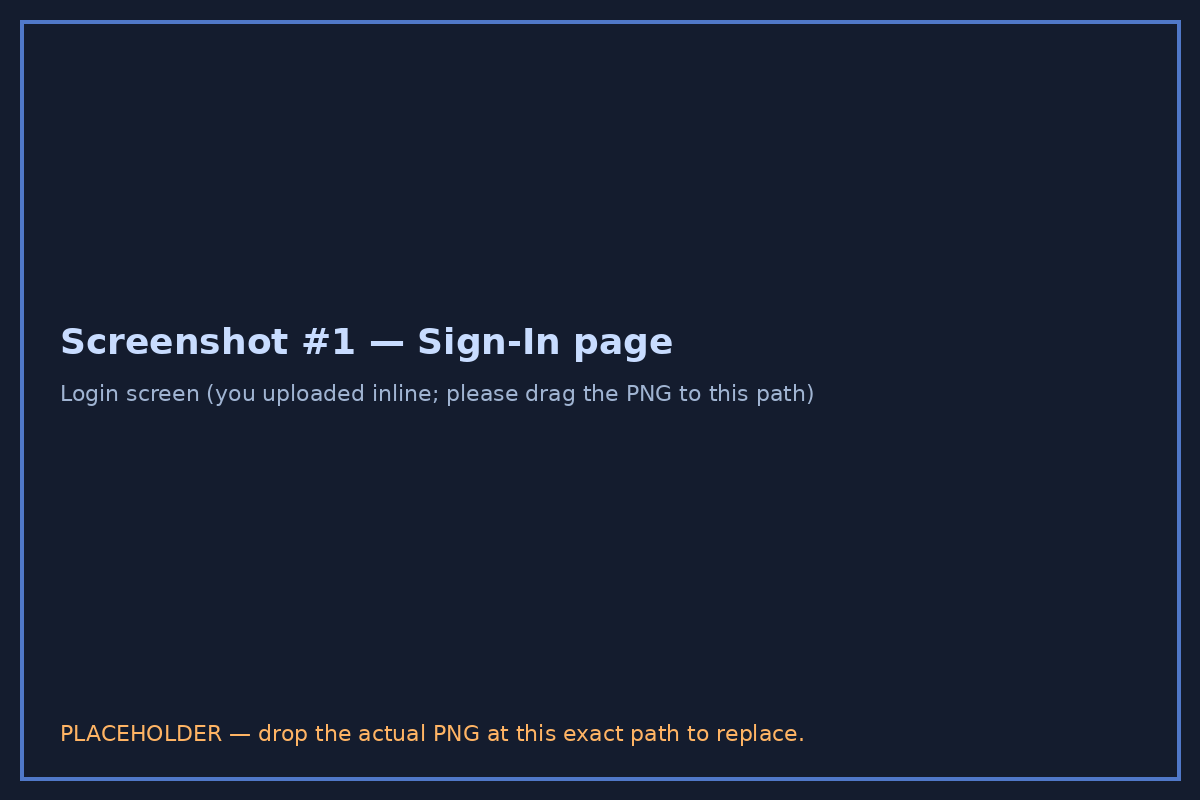
\includegraphics[width=0.31\textwidth,height=2.6cm,keepaspectratio]{figures/gui/gui_01_login.png}} &
\fbox{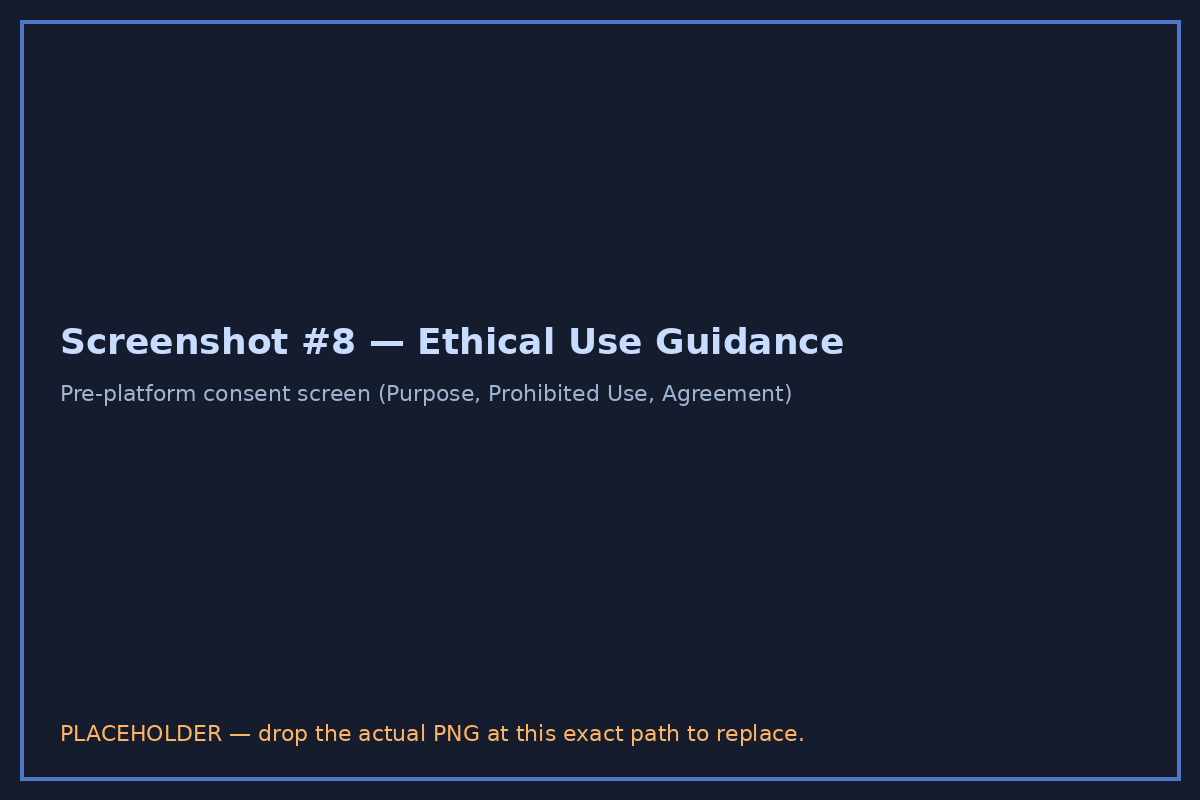
\includegraphics[width=0.31\textwidth,height=2.6cm,keepaspectratio]{figures/gui/gui_08_ethical_use.png}} &
\fbox{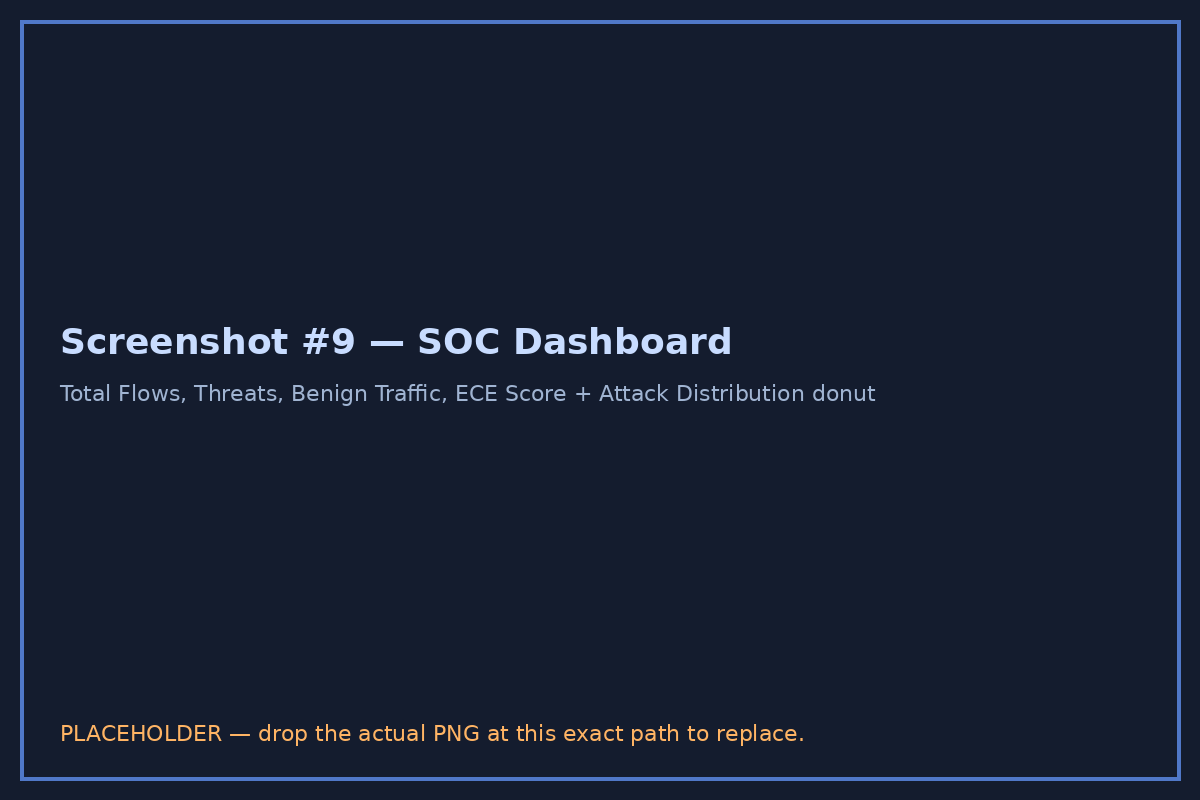
\includegraphics[width=0.31\textwidth,height=2.6cm,keepaspectratio]{figures/gui/gui_09_soc_dashboard.png}} \\
\scriptsize (a) Authentication &
\scriptsize (b) Ethical-use consent &
\scriptsize (c) SOC Dashboard \\[4pt]
\fbox{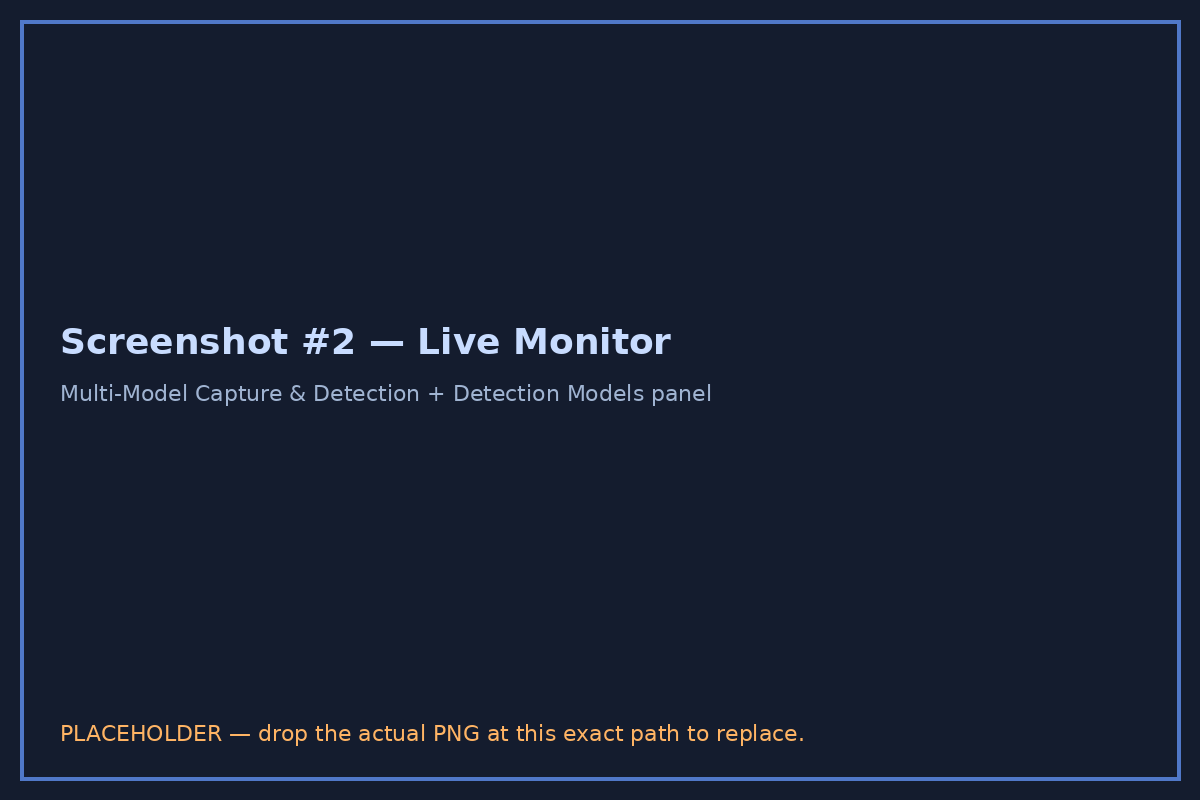
\includegraphics[width=0.31\textwidth,height=2.6cm,keepaspectratio]{figures/gui/gui_02_live_monitor.png}} &
\fbox{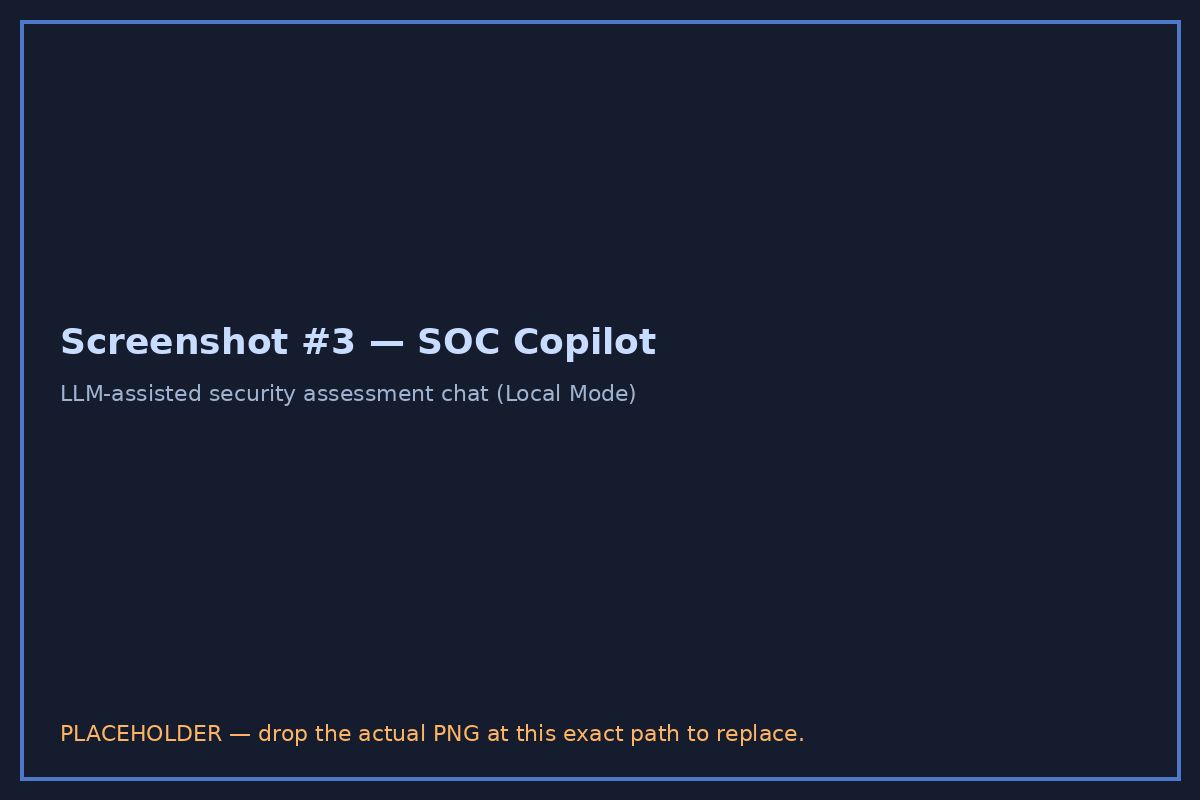
\includegraphics[width=0.31\textwidth,height=2.6cm,keepaspectratio]{figures/gui/gui_03_soc_copilot.png}} &
\fbox{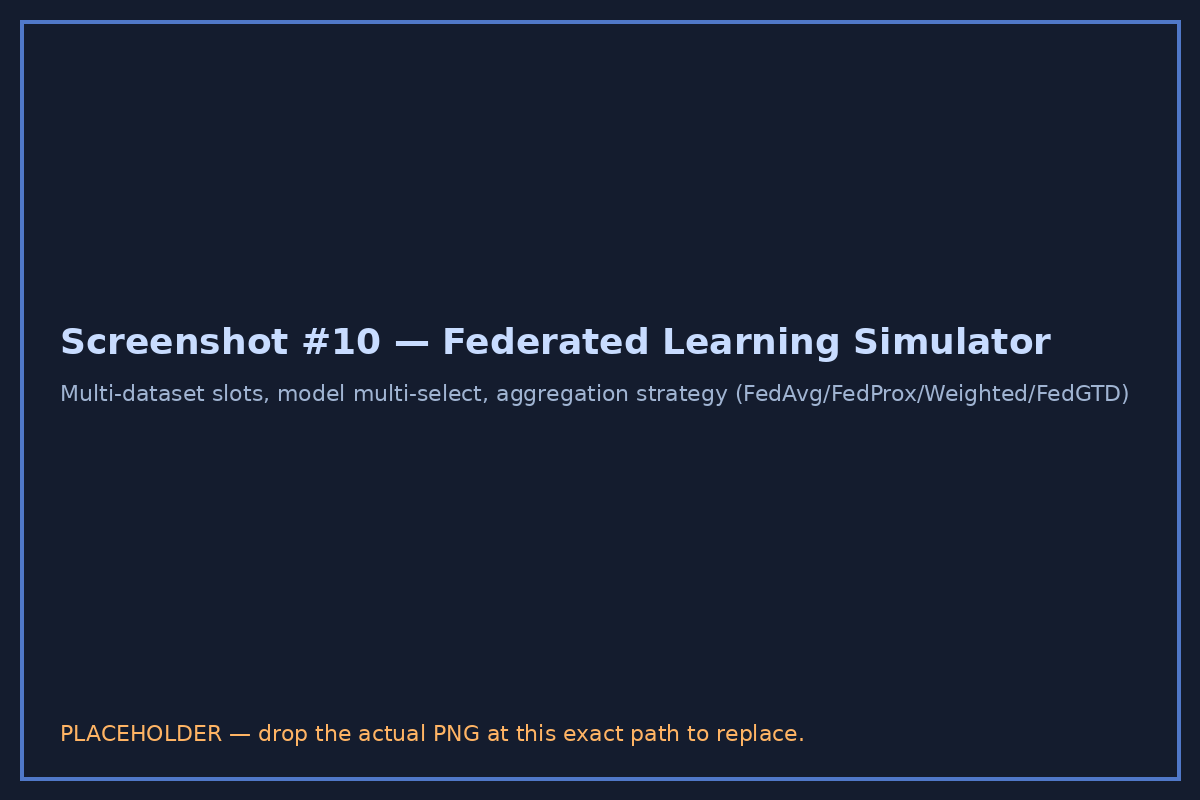
\includegraphics[width=0.31\textwidth,height=2.6cm,keepaspectratio]{figures/gui/gui_10_fed_learning.png}} \\
\scriptsize (d) Live Monitor &
\scriptsize (e) SOC Copilot (LLM assistant) &
\scriptsize (f) Federated Learning Simulator \\
\end{tabular}
\caption{Demonstration of practical operation of RobustIDPS.ai
(part~1)~--- from sign-in to distributed training:
\textbf{(a)}~Sign-In page with e-mail/password authentication and
new-user registration; \textbf{(b)}~``Ethical Use Guidance and
Consent'' page~--- mandatory acknowledgement of permitted
scenarios (academic research, authorised penetration testing,
government and defence research, evaluation and benchmarking) and
prohibited actions, implementing the MLSecOps requirement on
operator admission; \textbf{(c)}~SOC Dashboard page~--- summary
over 1{,}000 flows, 347 detected threats, 65.3\,\% benign-traffic
share, and the current calibration estimate ECE\,=\,0.043, with
the distribution across five severity levels and the canonical
attack-distribution and confidence histograms;
\textbf{(d)}~Live~Monitor page~--- starting a streaming capture
on the network interface \texttt{eth0} with selection of an
ensemble of seven detection models (SurrogateIDS, Neural~ODE,
Optimal~Transport, FedGTD, SDE-TGNN, CyberSecLLM, and others)
and the capture interval (5--120~s); \textbf{(e)}~SOC Copilot
page~--- the interactive LLM assistant in local mode answering
the analyst's query ``Get the Live Monitor results with breakdown
by threat, severity, and confidence'' against the real capture
session data; \textbf{(f)}~Federated Learning Simulator page~---
launching federated training over several datasets simultaneously
(CSV/PCAP slots Slot~1--3) with selection of the aggregation
strategy (FedAvg, FedProx, Weighted, FedGTD), IID/Non-IID regime,
and the differential-privacy option.}
\label{fig:gui_walkthrough_p1}
\end{figure}

\begin{figure}[htbp]
\centering
\setlength{\fboxsep}{0pt}\setlength{\fboxrule}{0.4pt}
\renewcommand{\arraystretch}{0.92}\begin{tabular}{@{}c@{\hspace{4pt}}c@{\hspace{4pt}}c@{}}
\fbox{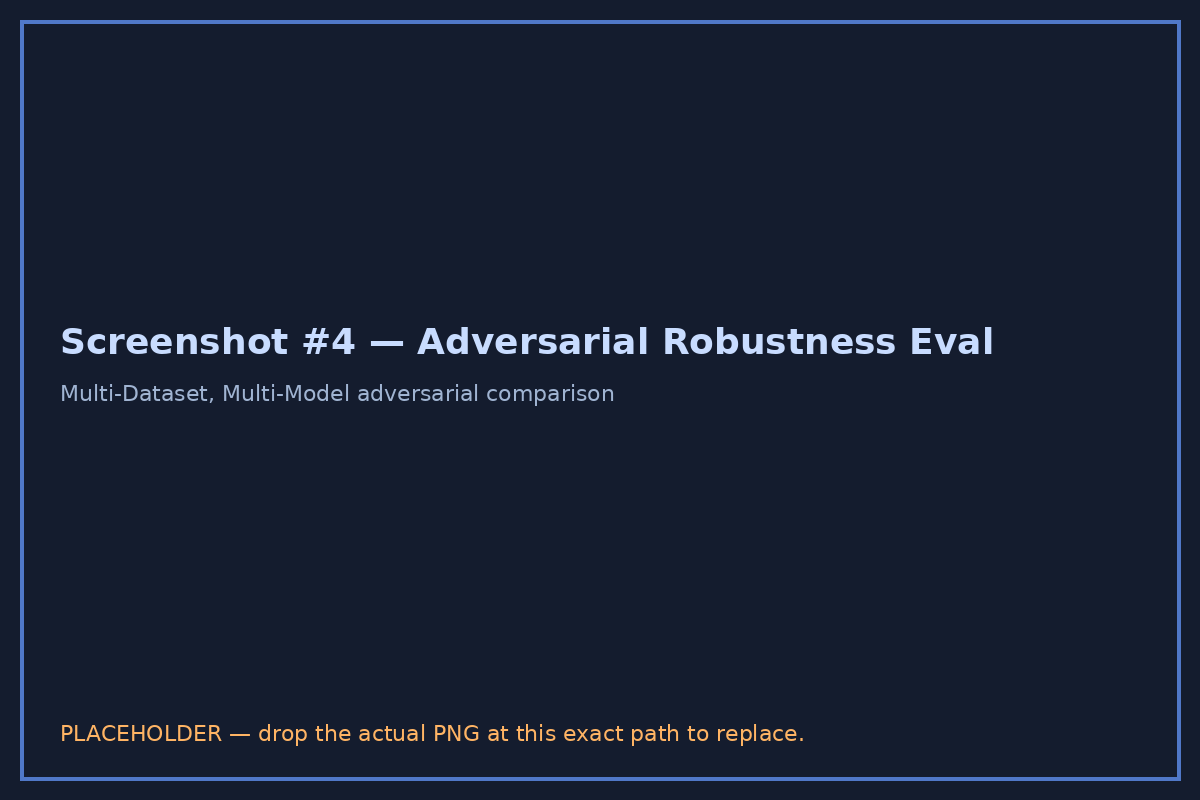
\includegraphics[width=0.31\textwidth,height=2.6cm,keepaspectratio]{figures/gui/gui_04_adversarial_eval.png}} &
\fbox{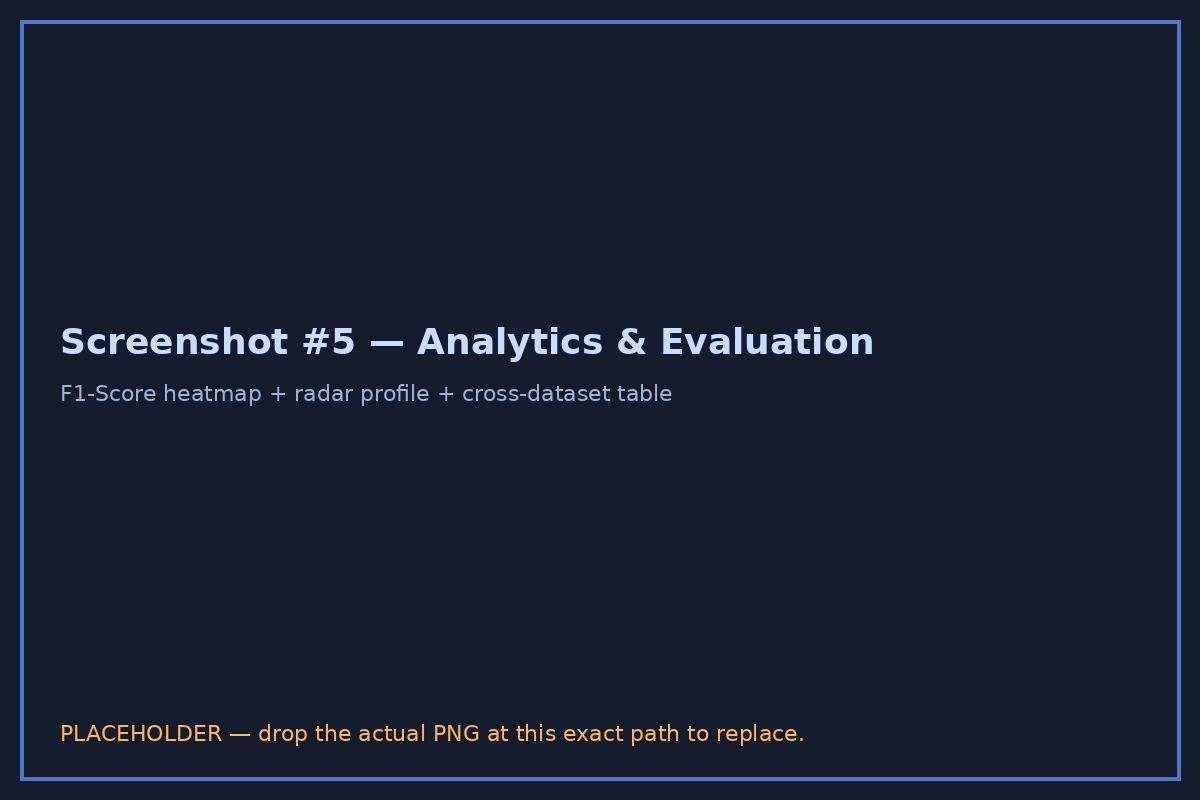
\includegraphics[width=0.31\textwidth,height=2.6cm,keepaspectratio]{figures/gui/gui_05_analytics_charts.png}} &
\fbox{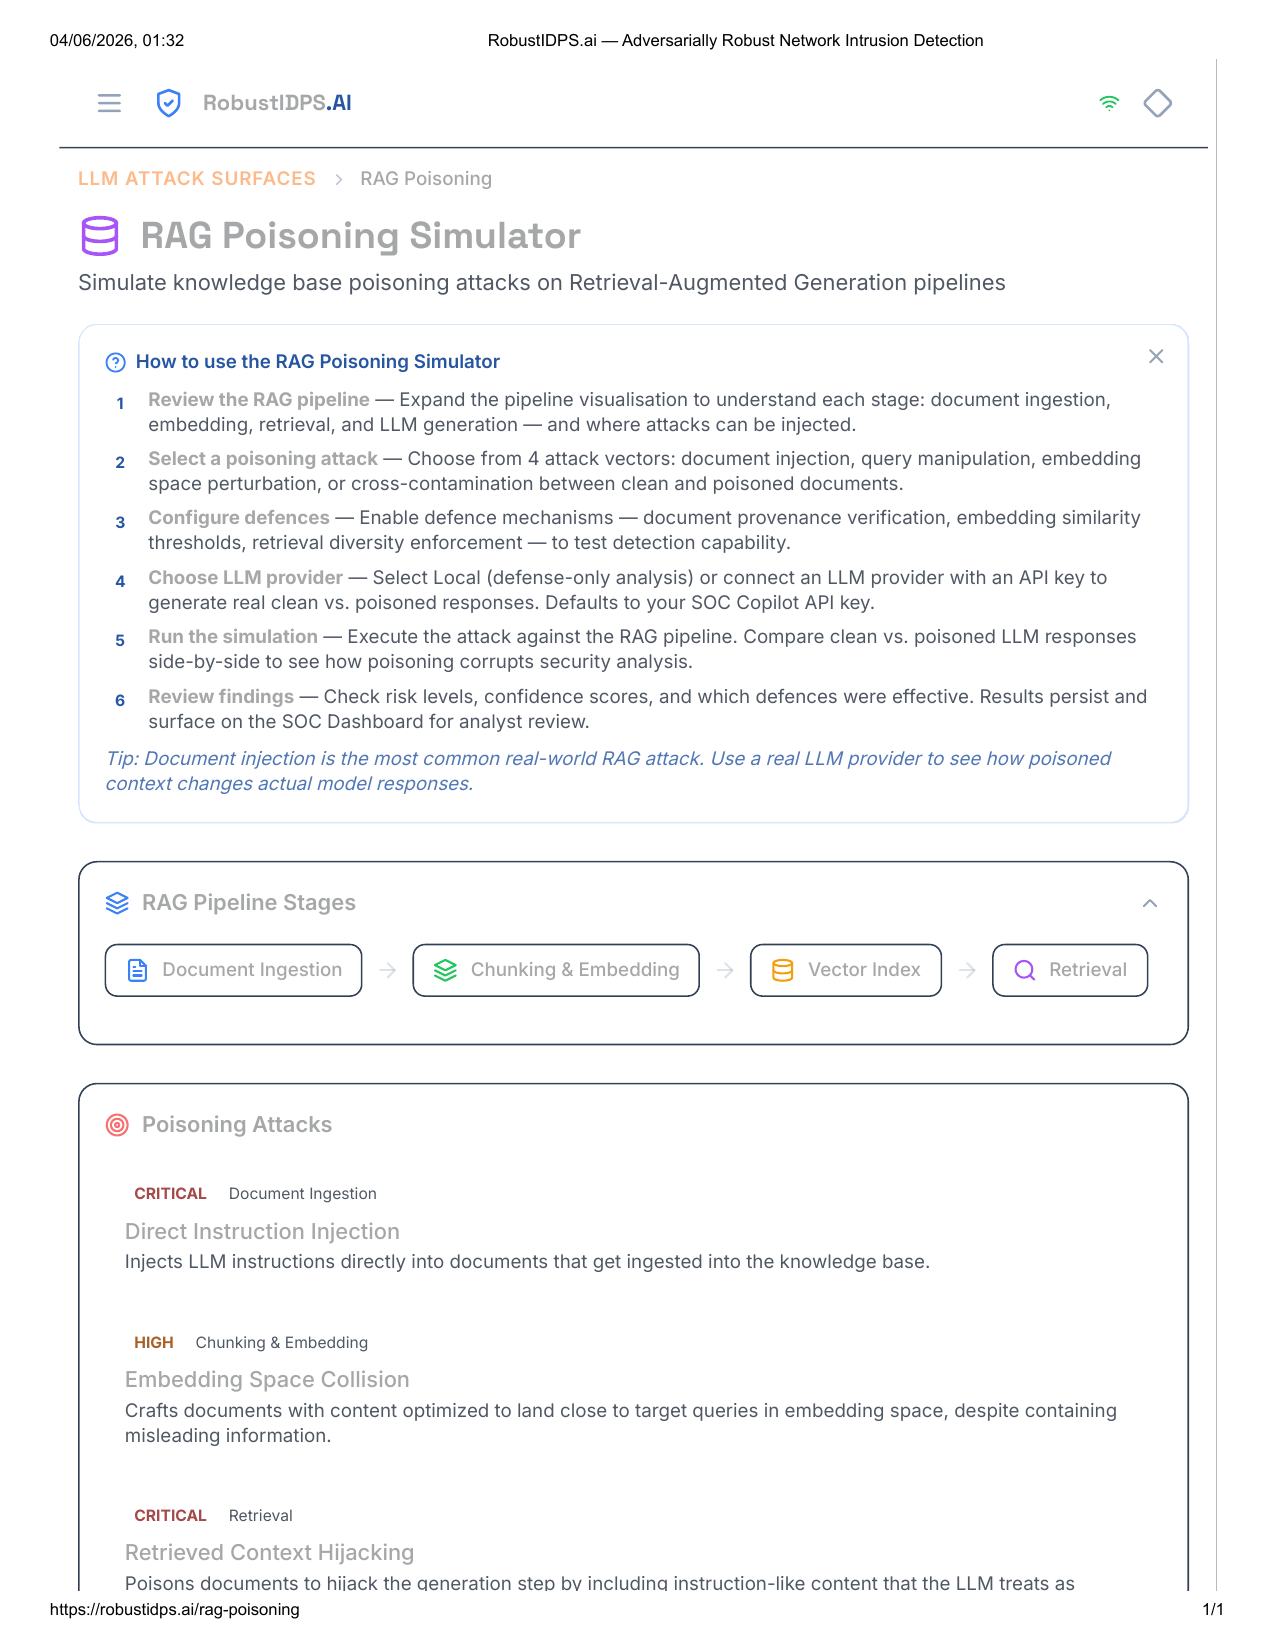
\includegraphics[width=0.31\textwidth,height=2.6cm,keepaspectratio]{figures/gui/gui_07_rag_poisoning.png}} \\
\scriptsize (g) Adversarial robustness comparison &
\scriptsize (h) Analytics and evaluation &
\scriptsize (i) RAG Poisoning Simulator \\
\end{tabular}
\caption{Demonstration of practical operation of RobustIDPS.ai
(part~2)~--- adversarial testing, analytics, and LLM attack
surfaces: \textbf{(g)}~Adversarial~Eval page~--- multi-dataset
comparison of models for robustness against six adversarial-attack
methods (FGSM, PGD, C\&W, DeepFool, Gaussian noise, Label masking);
\textbf{(h)}~Analytics \& Evaluation page~--- F1 metric comparison
for seven models across six benchmarks with a heatmap, a radar
profile, and a cross-dataset consistency table;
\textbf{(i)}~RAG Poisoning Simulator page~--- simulation of attacks
on the RAG pipeline of an LLM with four attack vectors (document
injection, query manipulation, embedding-space perturbation,
cross-contamination).}
\label{fig:gui_walkthrough_p2}
\end{figure}

\begin{figure}[htbp]
\centering
\fbox{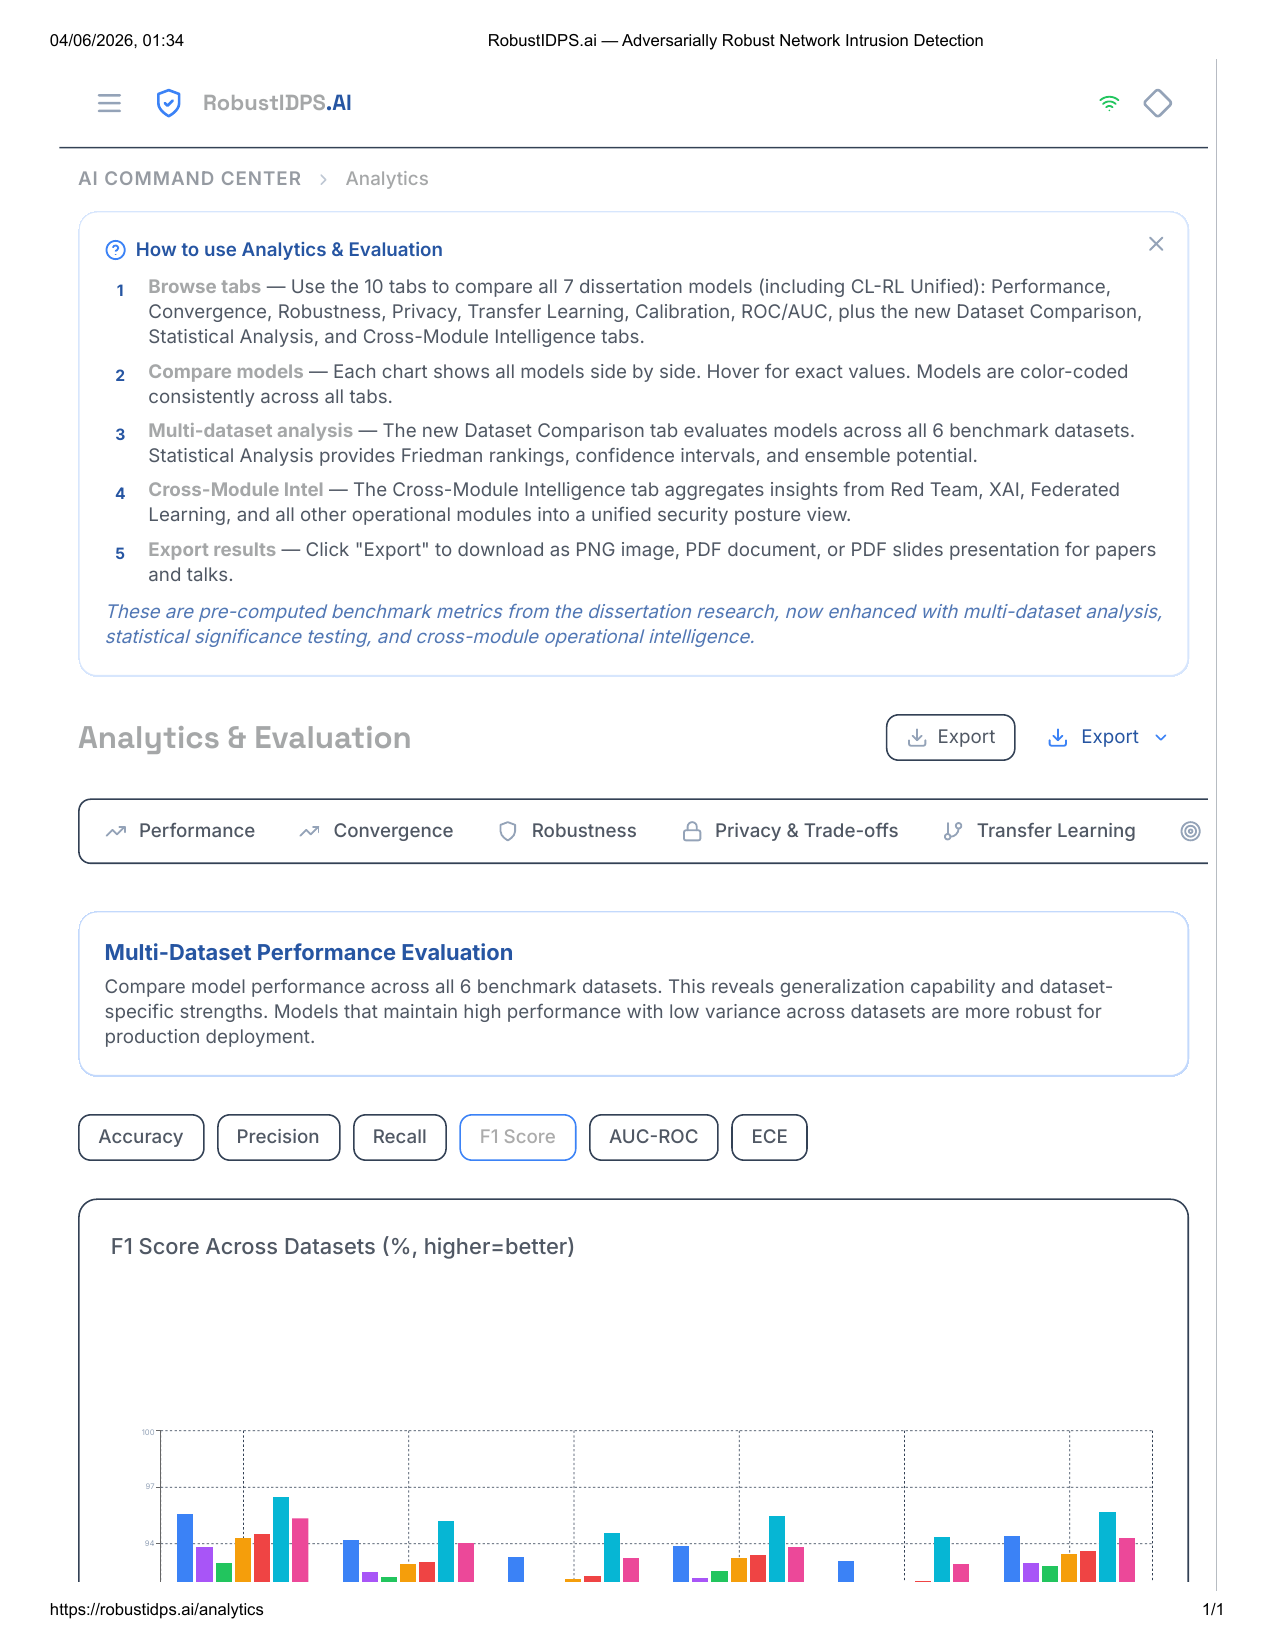
\includegraphics[width=0.86\textwidth]{figures/gui/gui_06_analytics_intro.png}}
\caption{The Analytics \& Evaluation page with the ``How to use''
hint open: interactive explanations of the ten comparative
model-evaluation tabs, with PNG/PDF export and a PDF presentation
export.}
\label{fig:gui_analytics_intro}
\end{figure}

%%=====================================================================
\section{Software Realisation of Models and Algorithms for Adversarially Robust Network Traffic Analysis}
\label{sec:features}
%%====

The software realisation of all seven models M1--M7 is organised as a Python package \texttt{robustidps} with the following file layout: models live in \texttt{robustidps/models/} as separate modules \texttt{ct\_tgnn.py} (M1), \texttt{fedllm\_api.py} (M2), \texttt{triplee\_tgnn.py} (M3), \texttt{mambashield.py} (M4), \texttt{sde\_tgnn.py} and \texttt{uc\_hgp.py} (M5/M6), \texttt{game\_theoretic.py} (M7), and \texttt{pq\_idps.py} (post-quantum module); the training pipeline lives in \texttt{robustidps/training/} with sub-modules \texttt{federated.py} (Byzantine-robust FL aggregation), \texttt{adversarial.py} (PGD/FGSM/C\&W), and \texttt{calibration.py} (temperature and Platt calibration); the inference pipeline lives in \texttt{robustidps/inference/} with batch and streaming implementations.

Key library dependencies are: \texttt{torch~2.2+} (core framework), \texttt{torch\_geometric~2.5+} with \texttt{torch\_geometric\_temporal~0.54} (graph operations and temporal layers), \texttt{torchdiffeq~0.2.4} (adaptive DOPRI5 Neural-ODE integration), \texttt{mamba\_ssm~1.2+} (selective state-space model for M4), \texttt{flwr~1.7+} (Flower as federated framework for M2), \texttt{geomloss~0.2.6} (Sinkhorn optimal-transport regularisers), and \texttt{pyOpenSSL} with PQClean bindings (Kyber, Dilithium, SPHINCS+) for post-quantum cryptography.

Representative training and inference invocations:
\begin{verbatim}
python -m robustidps.train --model ct_tgnn --dataset cic-iot-2023 \
       --epochs 100 --lr 2e-4 --hidden 256
python -m robustidps.train --model fedllm_api --num-clients 10 \
       --rounds 100 --dp-epsilon 0.85 --dp-delta 1e-5
python -m robustidps.train --model mambashield --state-dim 64 \
       --poison-min 0.05 --poison-max 0.3
python -m robustidps.eval --model-ensemble all --dataset unsw-nb15 \
       --attack pgd --eps 0.03
python -m robustidps.serve --port 8080 --batch-size 1024 \
       --device cuda:0
\end{verbatim}

Training uses AdamW with initial learning rate $2\times10^{-4}$, weight decay $10^{-5}$, and cosine annealing. Mixed-precision training (\texttt{torch.cuda.amp}) reduces memory by 40\%. Gradient clipping at norm 1.0 prevents instability. Early stopping with patience of 10 epochs monitors validation loss. Architectural details of models M1--M7 are not re-stated in this section and are given in Chapter~\ref{ch:methods}.

%%=====================================================================
\section{System Performance Optimisation}
\label{sec:hyperparams}
%%====

Table~\ref{tab:hyperparams} consolidates the principal hyperparameters for all methods as configured for the network-security domain. All values were selected through grid search on the CIC-IoT-2023 validation set and confirmed stable across the remaining five datasets.

\begin{table}[htbp]\centering\small
\caption{Consolidated hyperparameter configuration for all methods in the cybersecurity domain.}
\label{tab:hyperparams}
\small
\renewcommand{\arraystretch}{0.92}\begin{tabular}{p{3.5cm} p{2.5cm} p{2.5cm} p{5.0cm}}
\toprule
\textbf{Method} & \textbf{Parameter} & \textbf{Value} & \textbf{Rationale} \\
\midrule
\multirow{4}{3.5cm}{M1: CT-TGNN}
& Hidden dim & 256 & Capacity for 83-feature input \\
& ODE tolerance & $10^{-5}$ & Balance accuracy/speed \\
& Time constants & 1/60/3600\,s & Packet/session/campaign scales \\
& Lipschitz bound & Spectral norm & Certified robustness \\
\addlinespace
\multirow{4}{3.5cm}{M2: FedLLM-API}
& Clipping $C$ & 1.0 & DP sensitivity bound \\
& DP $(\epsilon,\delta)$ & $(0.85, 10^{-5})$ & Strong privacy guarantee \\
& OT reg $\lambda$ & 0.1 & Sinkhorn convergence \\
& LLM weight & 0.3 & Ensemble balance \\
\addlinespace
\multirow{3}{3.5cm}{M3: TripleE-TGNN}
& EWC $\lambda$ & 0.5 & Forgetting prevention \\
& Level weights & 0.4/0.3/0.3 & Service emphasis \\
& Consistency $\lambda_{\mathrm{con}}$ & 0.1 & Cross-level agreement \\
\addlinespace
\multirow{3}{3.5cm}{M4: MambaShield}
& State dim & 64 & SSM capacity \\
& Kernel length & 1024 & Sequence coverage \\
& Poison schedule & 0.05--0.3 & Progressive hardening \\
\addlinespace
\multirow{3}{3.5cm}{M5/M6: Stoch.Trans.}
& MC samples & 50 & Uncertainty quality \\
& Triage threshold & 0.3 & FP/FN balance \\
& Calibration & Temperature & ECE minimisation \\
\addlinespace
\multirow{2}{3.5cm}{M7: Certification}
& MWU $\eta$ & $\sqrt{\log|\calC|/T}$ & Optimal regret \\
& Unc. penalty $\kappa$ & 0.5 & Risk sensitivity \\
\bottomrule
\end{tabular}
\end{table}

Performance optimisation of the inference pipeline includes: (i)~ahead-of-time JIT compilation of graph modules via \texttt{torch.compile} with the \texttt{reduce-overhead} mode, yielding a $28\,\%$ latency reduction; (ii)~batched inference with dynamic buffering up to 1024 events and a $10\,$ms timeout, sustaining a throughput of $10\,$Gbit/s on a node equipped with an NVIDIA~A100 GPU; (iii)~mixed precision (\texttt{bfloat16} activations, \texttt{float32} normalisation) reducing GPU memory consumption by $40\,\%$; (iv)~Redis-cached graph snapshots with TTL $3600\,$s, eliminating redundant topology reconstructions under high-frequency queries. End-to-end latency from packet arrival to alert publication remains below $50\,$ms at the 99\textsuperscript{th} percentile.

%%=====================================================================
\section{Deployment and Integration Infrastructure of the System}
\label{sec:tech_stack_ui}
%%====

\subsection{Implementation Technology Stack}
\label{subsec:tech_stack}

The RobustIDPS.ai software platform is a \emph{single Progressive
Web Application} (PWA) split into a server-side and a client-side
tier, containerised with Docker~Compose and orchestrated by a unified
back-end / inference process. The stack has been chosen so as to
provide simultaneously: (i)~reproducible training and inference of
the deep graph-neural-network Models M1--M7; (ii)~resilient
streaming processing of real-time network traffic; (iii)~an
interactive SOC-analyst user interface; (iv)~integration with
external large-language-model (LLM) providers through a single
API-abstract layer.

\begin{enumerate}[leftmargin=2em, itemsep=0pt]
\item \textbf{Server tier (Python~3.11)}~--- an asynchronous
HTTP/WebSocket server on FastAPI (60+ REST API endpoints) on top
of which the model pipeline runs in PyTorch~2.x with PyTorch
Geometric and DGL extensions for graph operations; batch traffic
processing relies on NFStream for flow-feature extraction from
PCAP and on dpkt/Scapy for raw-packet parsing; service queues and
Pub/Sub are implemented in Redis~7 (cache + queue); persistent
storage of benchmarks and incident logs is PostgreSQL~16.

\item \textbf{Client tier (TypeScript / React~18)}~--- a
Progressive Web Application of \textbf{51~user-interface pages}
organised into ten functional groups (see
Section~\ref{subsec:func_incident}). Real-time updates of
streaming classifications are pushed over WebSocket; graph and
metric visualisations use Recharts and a bespoke D3.js graph
visualisation; styling is Tailwind~CSS with a dark theme by
default.

\item \textbf{LLM integration tier}~--- a single LLM-provider
abstraction with implementations for four commercial back-ends
(Anthropic Claude, OpenAI GPT-4o, Google Gemini, DeepSeek) and a
local-inference back-end; the four-level LLM defence (Prompt
Injection, Jailbreak, RAG Poisoning, Multi-Agent Chain) is
implemented as a transparent middleware between UI and providers.

\item \textbf{Deployment tier}~--- Docker containerisation with
multi-stage builds and Compose orchestration; integration with
existing information-security tooling is provided by a plug-in
for the Suricata EVE-JSON format, which allows RobustIDPS.ai to
be embedded into the operating IDS of an organisation without
modifying existing signature rules (confirmed by the NII~IKT~LLC
implementation act, see Chapter~\ref{ch:platform}).

\end{enumerate}

\subsection{Used Packages and Versions}
\label{subsec:packages_versions}

Table~\ref{tab:packages_versions} lists the key software
dependencies of the RobustIDPS.ai platform with the versions used
to produce the experimental results and to sign the implementation
acts. The complete \texttt{requirements.txt} and
\texttt{package.json} are deposited with the source code on Zenodo
(DOI: 10.5281/zenodo.19129512).

\begin{table}[H]
\centering
\caption{Software dependencies of the RobustIDPS.ai platform.}
\label{tab:packages_versions}
\small
\renewcommand{\arraystretch}{0.92}\begin{tabular}{@{}lll@{}}
\toprule
\textbf{Category} & \textbf{Package} & \textbf{Version} \\
\midrule
Implementation language & Python & 3.11.x \\
Web server & FastAPI & 0.110+ \\
ASGI server & Uvicorn (uvloop) & 0.27+ \\
Deep learning & PyTorch & 2.2+ \\
Graph operations & PyTorch~Geometric & 2.5+ \\
Graph operations (alt.) & DGL & 2.1+ \\
Neural ODEs & torchdiffeq & 0.2.4 \\
State-space models & mamba-ssm & 1.2+ \\
Flow-feature extraction & NFStream & 6.5+ \\
Raw-packet parsing & dpkt~/~Scapy & 1.9~/~2.5 \\
Persistent store & PostgreSQL & 16 \\
Cache and queues & Redis & 7 \\
Containerisation & Docker & 24+ \\
Orchestration & Docker Compose & v2 \\
Client (language) & TypeScript & 5.3+ \\
Client (framework) & React & 18 \\
Client build & Vite & 5 \\
UI library & Tailwind CSS & 3.4 \\
Chart visualisation & Recharts & 2.10 \\
Graph visualisation & D3.js & 7 \\
Real-time updates & WebSocket (RFC~6455) & --- \\
LLM providers (APIs) & anthropic, openai, google-genai, deepseek & current \\
Signature plug-in & Suricata EVE-JSON & 7.0 (compat.) \\
\bottomrule
\end{tabular}
\end{table}

The presented technology stack ensures the integrity of the system realisation: integration into operational information-security tooling is confirmed by the implementation acts of NII~IKT~LLC (active use of the platform by in-house cybersecurity specialists) and Ksyrix~LLC (integration into the operating network-traffic analysis and infrastructure-protection system).

%%=====================================================================
\section{Comparative Analysis of Architectural and Functional Capabilities of RobustIDPS.ai versus Existing Intrusion Detection Systems}
\label{sec:integrated_arch}
%%====

The seven methods (M1--M7) are integrated into a unified detection pipeline whose data flow proceeds as follows. Raw network traffic enters through a data ingestion module that performs protocol parsing, flow extraction, and 83-feature computation. The CT-TGNN module constructs the temporal graph and computes continuous-time node embeddings. The TripleE-TGNN module maintains multi-level embeddings for hierarchical environments. The MambaShield module processes sequential event records for drift-adaptive scoring. The Stochastic Transformer and UC-HGP modules provide calibrated uncertainty estimates. All outputs feed into a decision engine that applies the game-theoretic strategy from the M7 Certification framework, producing alerts classified by severity and confidence. The FedLLM-API module enables periodic model synchronisation across organisational boundaries.

\begin{figure}[htbp]
\centering
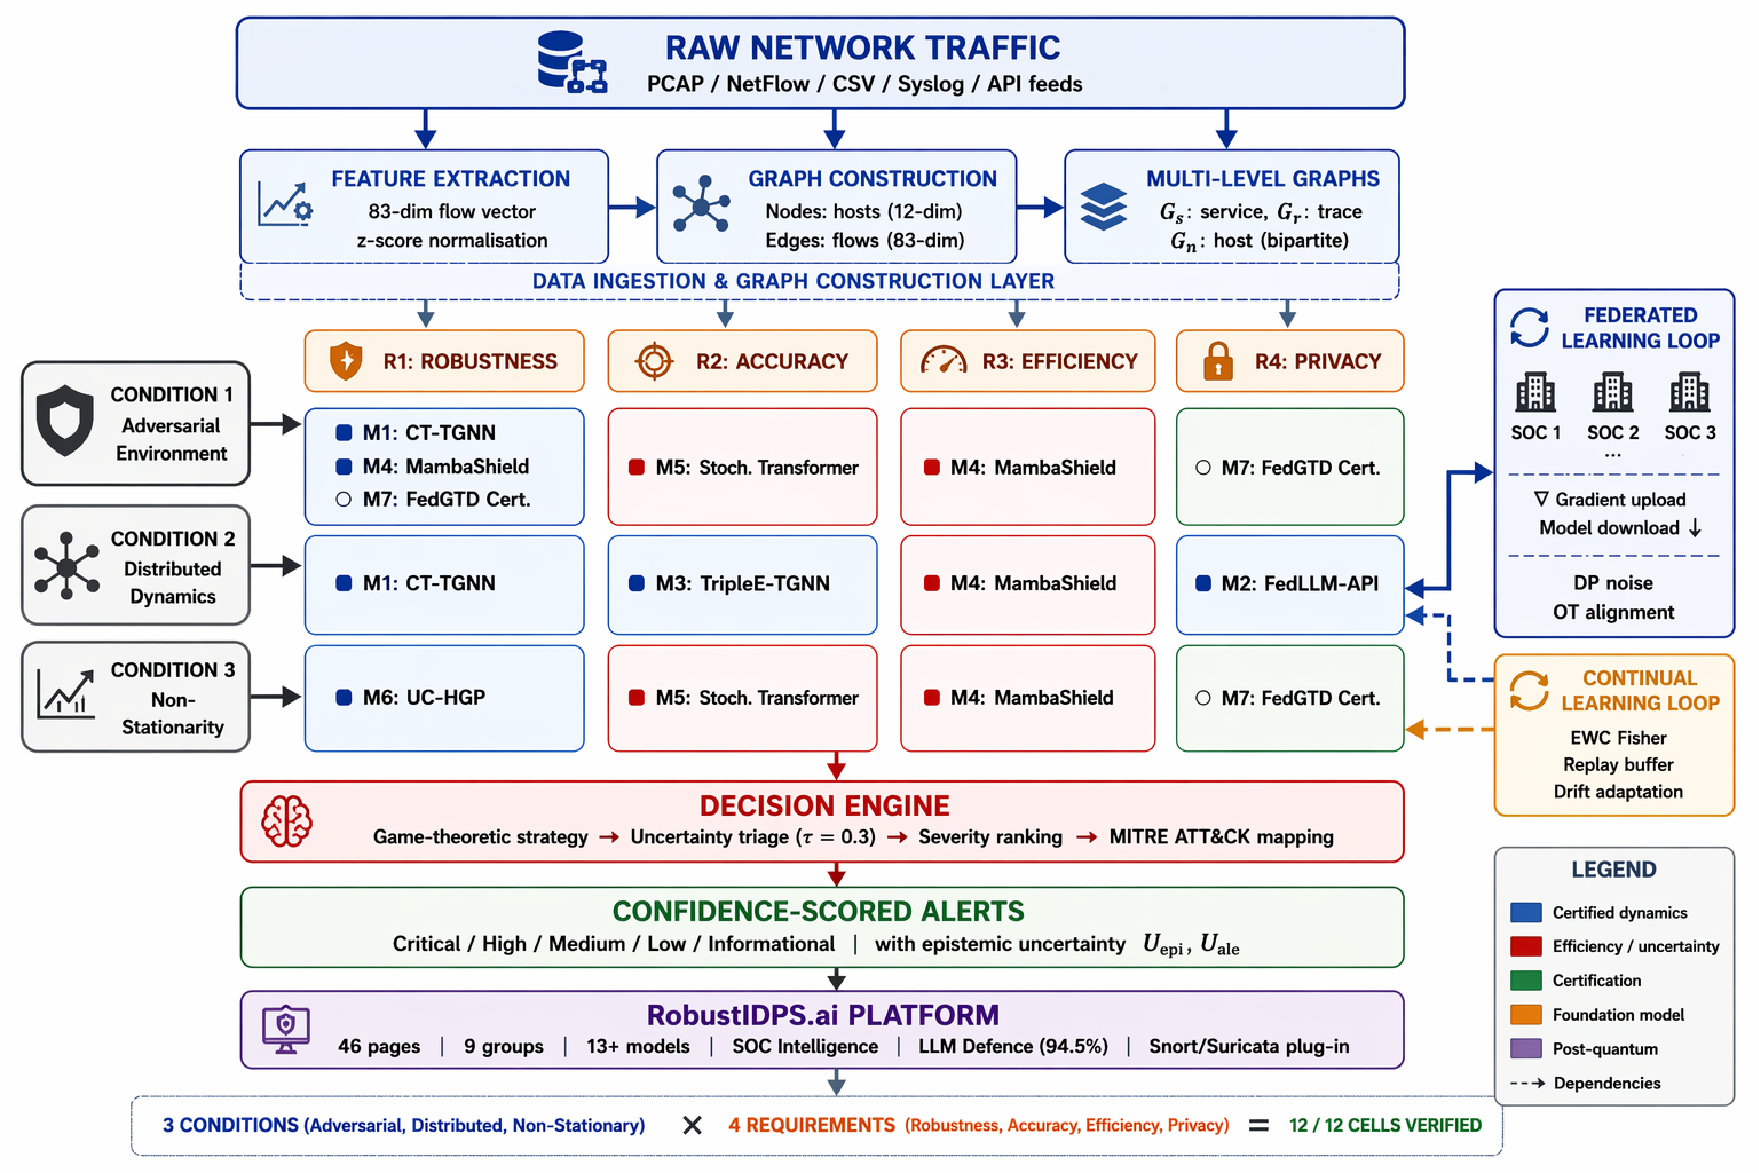
\includegraphics[width=0.85\textwidth]{figures/Main_arch_v1b.pdf}
\caption{Integrated detection pipeline showing the data flow from raw network traffic through all seven methods to severity-ranked, confidence-scored alerts. The FedLLM-API module synchronises models across boundaries under differential privacy.}
\label{fig:u_idps_arch}
\end{figure}

The system is designed for deployment as a plug-in for existing IDPS frameworks such as Snort~3~\cite{Roesch1999} and Suricata, consuming their alert feeds as additional input and producing enriched, confidence-scored outputs. The full software implementation is described in Chapter~\ref{ch:platform}, publicly archived under DOI 10.5281/zenodo.19129512~\cite{Anaedevha2026robustidps}.

%%=====================================================================

%%=====================================================================
%%   BENCHMARK VALIDATION OF THE HYBRID IDPS SYSTEM ON NETWORK TRAFFIC
%%   (Moved from former Chapter~4 \S\S4.1-4.5 as part of the Phase 2.5
%%   Option-B reorganisation: NIDS instantiation and its benchmark
%%   validation now sit together in one chapter.)
%%====

% Bridging paragraph before the methodology.
\medskip
\noindent\emph{Bridge with the above:}
Sections~\ref{sec:nidps_context}--\ref{sec:integrated_arch}
have shaped the instantiation of the Hybrid~IDPS system for the
network-traffic protection task at the level of entities, features,
hyperparameters, and integrated architecture.
Sections~\ref{sec:exp_methodology}--\ref{sec:ablation} below
systematically validate this realisation of the system on six
benchmark datasets, providing a direct mapping from results to the
invariants~P2--P6 from \S\ref{subsec:six_properties}.

%%=====================================================================

%%=====================================================================
\section{Ensuring Reproducibility of Results and Distribution of the Software Complex}
\label{sec:reproducibility}

Reproducibility of the dissertation's results is ensured by complete
deposition of source code, trained models, and experimental protocols in
the open Zenodo repository (DOI:~10.5281/zenodo.19129512).

\textbf{Source-code publication.} All RobustIDPS.ai components, including
17 neural-network models, server-side tier (FastAPI/Python), client-side
tier (React/TypeScript), and Suricata EVE-JSON plug-in, are released under
an open licence. The complete \texttt{requirements.txt} (Python) and
\texttt{package.json} (Node.js) with pinned dependency versions are
deposited alongside the code.

\textbf{Component descriptions.} Each component is accompanied by a
technical description of interfaces, input/output data formats, startup
parameters, and dependencies, structured as \texttt{README.md} and a
\texttt{docs/} directory split by functional group.

\textbf{Documentation and experiment-reproduction tools.} Scripts and
Makefile targets enable single-command launch of all key experiments on
benchmark datasets; hyperparameter configurations, dataset splits, and
evaluation parameters are pinned in YAML files.

\textbf{Open-source contributions.} Derived results with stand-alone value
beyond the dissertation (Suricata EVE-JSON plug-in, PyTorch~Geometric
wrappers for continuously evolving graphs) are submitted to the
corresponding upstream projects as pull requests.
%%====
\section{Conclusions for Chapter 3}
\label{sec:ch3_summary}
%%====

This chapter has systematically developed and software-implemented
the \textbf{RobustIDPS.ai} system as a NIDS-sector instantiation of
the Hybrid~IDPS mathematical model from
Chapter~\ref{ch:methods}. The chapter is \emph{strictly software-development
oriented}: the experimental investigation of the developed system
and its quantitative validation on benchmark datasets are reported
in Chapter~\ref{ch:experiments}.

Key software-engineering contributions of this chapter:
\begin{itemize}\setlength\itemsep{2pt}
\item \emph{(1)}~A formal pipeline for transforming raw PCAP and
CSV traffic into temporal graph structures with 12-dimensional
node features and 83-dimensional edge features, systematically
implementing the components $(\calV_t, \calE_t, X_t, A_t)$ of the
Hybrid IDPS tuple~\eqref{eq:hybrid_idps_tuple}.
\item \emph{(2)}~A unified 34-class classification taxonomy across
seven attack categories, extensible via LLM zero-shot classification.
\item \emph{(3)}~A comprehensive 83-feature engineering pipeline
covering flow statistics, inter-packet-interval distributions, flag
indicators, payload statistics and derived ratios.
\item \emph{(4)}~A NIDS-oriented software realisation of all seven
models M1--M7 with hyperparameters, time constants and architectural
configurations tailored to the network-traffic protection sector.
\item \emph{(5)}~A unified integrated system architecture providing
end-to-end flow from raw traffic to SOC analyst alerts with
confidence estimation and automated response.
\item \emph{(6)}~A production-grade technology stack
(FastAPI/PyTorch~2.x with PyTorch~Geometric and DGL extensions,
React~18 PWA, PostgreSQL~16, Redis~7, Docker~Compose), including
integration with four commercial LLM providers and a Suricata
EVE-JSON plug-in.
\item \emph{(7)}~A 51-page progressive web application user
interface aggregating 17 neural-network models into 10 functional
groups; a representative SOC analyst workflow is demonstrated.
\end{itemize}

The complete set of implemented components constitutes the
\textbf{RobustIDPS.ai} platform, deposited in the Zenodo
repository (DOI: 10.5281/zenodo.19129512) with open source code.
\emph{The quantitative experimental validation of the developed
system~--- detection quality assessment, adversarial robustness,
efficiency, privacy, calibration, ablation studies and cross-domain
transfer~--- is presented in Chapter~\ref{ch:experiments}.}

\noindent\textbf{Adaptation strategy across the seven methods.} The seven mathematical methods of Chapter~\ref{ch:methods} are adapted to the NIDS sector through a single principle: the abstract graph object $(\calV,\calE,X,A)$ is instantiated by replacing nodes with hosts and services, edges with network flows, node features with the 12-dimensional host-state vector, and edge features with the 83-dimensional flow-feature vector. The remaining mathematical apparatus~--- continuous-time integration, Lipschitz-bounded vector fields, Wasserstein alignment, selective state-space inference, hierarchical Gaussian processes, and Stackelberg games~--- transfers unchanged. This invariance is the technical pre-condition that allows the same Methods M1--M7 to be reused in Chapter~\ref{ch:uav} for the UAV-protection sector by simply re-instantiating the graph object: nodes become onboard sensors, edges become inter-sensor communication links, node features become per-sensor telemetry vectors, and edge features become link-quality statistics. The mathematical guarantees~--- certified Lipschitz radii, $(\varepsilon,\delta)$-differential-privacy budgets, PAC-Bayesian bounds, and no-regret regret bounds~--- carry over without modification, confirming the domain-independence claim of Chapter~\ref{ch:methods}.

\noindent\textbf{Operational scenarios and SOC-analyst workflow.} The platform supports five operational scenarios. \emph{Real-time monitoring}: WebSocket-streamed flow records are classified by the SurrogateIDS ensemble, with high-confidence alerts pushed to the Tier~1 analyst console and high-uncertainty alerts routed to the SOC Copilot for agentic investigation. \emph{Forensic analysis}: PCAP files uploaded through the drag-and-drop interface are processed offline through the full M1--M7 pipeline, with per-flow attribution traceable to MITRE ATT\&CK~\cite{Hernandez2015} techniques. \emph{Adversarial-robustness testing}: the red-team arena runs configurable attack families (FGSM, PGD, C\&W, DeepFool, HopSkipJump, BoundaryAttack) against any combination of the 17 models with reporting of certified-radius regressions. \emph{Federated training}: the Federated Learning page coordinates Byzantine-resilient training across registered participants with explicit $(\varepsilon,\delta)$-privacy accounting per round. \emph{Continual-learning calibration}: the Drift Monitor module compares the live traffic distribution against the training reference and triggers EWC-protected incremental updates when the Gaussian-process test fires. The five scenarios together provide a complete end-to-end coverage of the NIDS-sector operational requirements.
